\section{Application Layer}

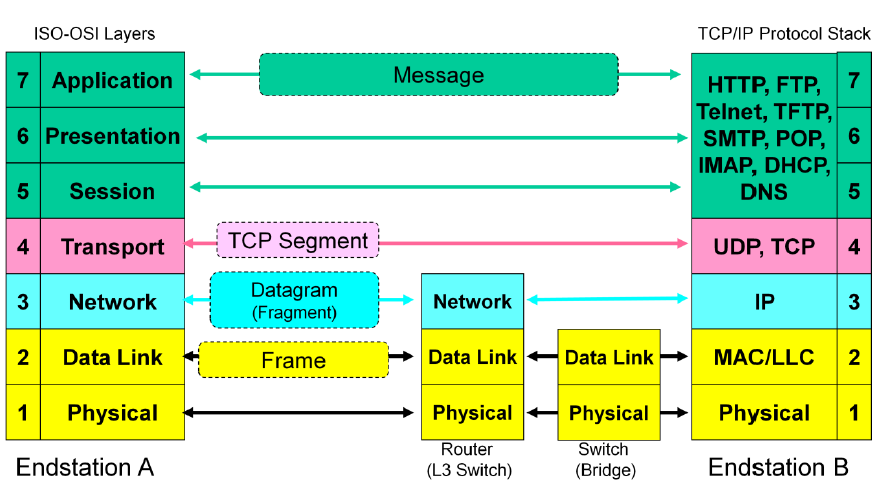
\includegraphics[scale=0.5]{media/osimodel.png}

\subsection{DNS}
Rekursive Abfrage: Server führt alle notwendigen Subqueries zur vollständigen Auflösung aus.\\\\
Nich-Rekursive Abfrage: Server liefert nur den nächsten zuständigen Name Server. Nach dem Prinzip "Frag einmal dort nach".\\
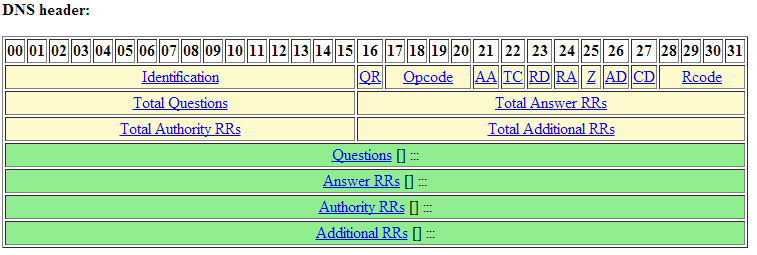
\includegraphics[scale=0.8]{media/DNSHeader.png}

\subsection{FTP}
Aktiv: Der Server baut die Datenkanal-Verbindung zum Client auf\\
Passiv: Der Client baut die Verbindung für den Datenkanal zum Server auf. Der Server ist nur "listening".\\
\textbf{Beispiel Verbindung} \\
USER jonas\\
PASS jonas\\
PASV\\
227: Entering Passive Mode (xxx,xxx,xxx,xxx,y, z)\\
//Port = 256*y+z\\
LIST\\
\\
\textbf{File Transfer Mode}\\
Im ASCII Mode werden die CR/LF für die jeweilige Zielplattform konvertiert.
Im Binary Mode wird nichts konvertiert.

\subsection{HTTP}
Persistent HTTP: keep-alive Header, TCP Verbindung behalten für mehrere Requests\\
Conditional Get: \\
\textbf{ETag:} \\Bei der ersten Anfrage einer Ressource sendet der Server einen für diese Ressource spezifischen ETag-Wert im ETag-Header-Feld, der vom Client zusammen mit der Ressource lokal gespeichert wird. (Abb.1) Bei einer erneuten Anfrage derselben Ressource sendet der Client in dem Header-Feld If-None-Match den zuvor gespeicherten ETag-Wert mit. (Abb.2) Auf der Server-Seite wird nun der gesendete ETag-Wert mit dem aktuellen verglichen und bei Übereinstimmung mit dem Statuscode 304 beantwortet. (Abb.3) Die Daten der Ressource werden in diesem Fall nicht mitgeschickt und der Client verwendet die lokal gespeicherten Daten.\\\\
\textbf{Headers für Cache Control:}\\
if-match\\
if-none-match\\
if-modified-since\\
if-range\\\\

